\section{Analisi}
In questa prima sezione si analizzano le motivazioni e le specifiche necessarie per la realizzazione del progetto. Verranno inoltre illustrati i requisiti e i diagrammi necessari per illustrare il comportamento del sistema.
\subsection{Obiettivi}
Nel ventunesimo secolo l'informatica ha compiuto passi da gigante, insinuandosi in ogni branca del sapere scientifico. Questo ha portato ad espandere il sapere conoscitivo in maniera esponenziale e ad oggi non è più possibile avere una conoscenza totalitaria del settore. Di conseguenza esistono tantissime figure specializzande nei più disparati settori ed è difficile individuare con precisione quale debba essere il percorso formativo necessario per il raggiungimento della carriera desiderata. A partire da questi propositi nasce \textbf{PocketDev} un applicativo che guida l'utente nel percorso formativo utile a comprendere i requisiti teorici e pratici per conseguire la carriera desiderata.
\subsection{Panoramica}
Il sistema mantiene delle informazioni legate ad una carriera IT. Ad ogni carriera è associato un percorso formativo che consiste in una serie di concetti che possono essere di natura teorica o pratica. I primi riguardano argomenti inerenti alla teoria dell'informazione, mentre i secondi rappresentano gli strumenti che si possono imparare e che devono essere applicati insieme alla teoria per poter lavorare.
\subsection{Requisiti Funzionali}
\begin{center}
\begin{tabular}{|l|l|}
\hline
\textbf{Codice} & \textbf{Nome Requisito}\\ 
\hline
RF\_01 & Mostra Carriere IT\\
\hline 
RF\_02 & Mostra Percorso Carriera\\
\hline
RF\_03 & Mostra Info Carriera\\
\hline
RF\_04 & Mostra Guida Percorso\\
\hline
RF\_05 & Mostra Libri Percorso \\
\hline
\end{tabular}
\end{center}
\begin{description}
 \item [RF\_01: Mostra Carriere IT:] Il sistema mostra l'insime delle carriere informatiche disponibili;
 \item[RF\_02: Mostra Percorso Carriera:] Il sistema mostra i requisiti teorici e pratici necessari per il conseguimento della carriera;
 \item[RF\_03: Mostra Info Carriera:] Il sistema mostra delle informazioni generiche sulla carriera IT mostrando una descrizione di base ed altre informazioni;
 \item[RF\_04: Mostra Guida Percorso:] Il sistema mostra una guida breve sui concetti di base di un percorso formativo.
 \item[RF\_05: Mostra Libri Percorso:] Il sistema mostra una serie di libri utili ad approfondire un percorso formativo
\end{description}
\subsection{Requisiti Non Funzionali}
Per quanto concerne i requisiti non funzionali gli attributi su cui si focalizzerà il sistema finale sono:
\begin{itemize}
 \item \textbf{Usabilità:} il sistema dovrà essere il più semplice ed intuitivo possibile per l'utente finale;
 \item \textbf{Efficienza:} il sistema dovrà rispondere in brevi lassi di tempo.
\end{itemize}
\subsection{Diagramma dei Casi d'Uso}
\begin{figure}[H]
 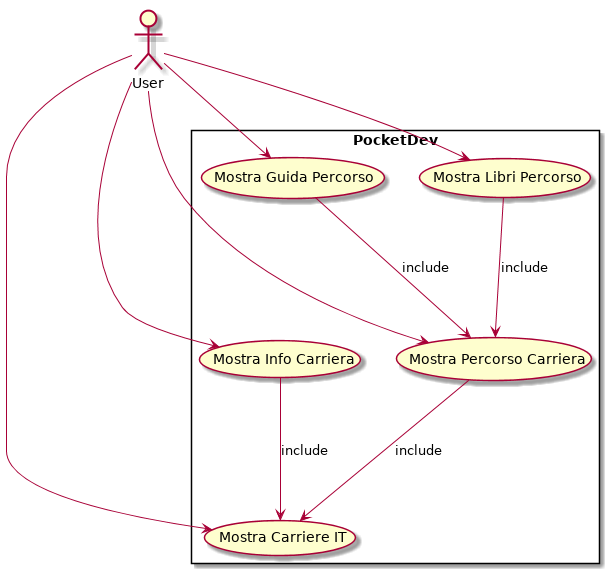
\includegraphics[scale=.5]{usecase.png}
\end{figure}
\subsection{Mockup}
Il sistema presenta un'unica pagina web che contiene tutte le interazioni necessarie tra il sistema e l'utente. Durante il click della combo box il sistema recupera le informazioni necessarie sul percorso formativo della singola carriera mostrandole in un widget di tipo albero. Cliccando su ogni elemento si aggiorna il pannello vicino che suddivide le informazioni in 3 tipi: informazioni generali, una breve guida, se presente, e un insieme di libri da acquistare per approfondire.
\begin{figure}[H]
\begin{center}
 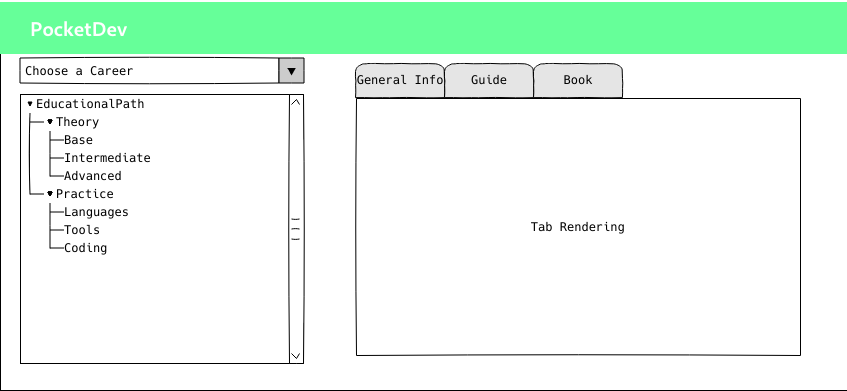
\includegraphics[scale=.4]{mockup.png}
\end{center}
\end{figure}
